\documentclass{article}
\usepackage[preprint]{neurips_2024}
\usepackage[utf8]{inputenc}
\usepackage[T1]{fontenc}
\usepackage[hidelinks]{hyperref}
\usepackage{url}
\usepackage{booktabs}
\usepackage{amsfonts}
\usepackage{amsmath}
\usepackage{amssymb}
\usepackage{nicefrac}
\usepackage{microtype}
\usepackage{graphicx}
\usepackage{xcolor}
\usepackage{enumitem}
\graphicspath{{figs/}}
\newcommand{\kstar}{k^{\ast}}
\newcommand{\ddecl}{d_{\mathrm{decl}}}
\input{numbers}

\title{Binding Capacity Tracks the Pretraining Recipe, Not Scale Alone}

\author{%
  Manas Venkata Sai Ravulapalli\\
  Efficient Computation Inc.\\
  \texttt{manas@perseus.so}
  \And
  Samrath Chadha\\
  Efficient Computation Inc.\\
  \texttt{samrath@perseus.so}
}

\begin{document}
\maketitle

\begin{abstract}
How many entity--attribute bindings can a language model hold in context before recall collapses? We measure
this capacity, $\kstar$, on a single controlled binding task across \NModelsRaw{} open models, and find it is not a
scaling law. After excluding one model whose single-binding accuracy is already at chance (its inclusion would inflate the reported range), $\kstar$ spans $\KstarMin$ to $\KstarMax$, an $\KstarRangeFactor\times$ range, and tracks the
pretraining \emph{recipe}: the median is $\KstarOldMed$ for pre-2023 recipes and $\KstarModMed$ for modern ones. Because \NModelsRaw{} models
are only \emph{ten families}, we report every comparison twice: at the model level, as a reader would compute
it from the released table, and then under a bootstrap clustered on families. The capacity difference
survives (family-clustered $95\%$ CI of the median difference $\KstarFamCI$, family-level $p=\KstarFamP$).
Scale alone does not buy capacity (the Pythia ladder holds $\kstar\in[\PythiaKstarLo,\PythiaKstarHi]$ from 410M to 12B) while scale
\emph{within} a modern recipe does, so capacity is a recipe$\,\times\,$scale interaction. Alignment leaves it
untouched. We then ask what the recipe controls geometrically, and report a negative result:
of the two non-tautological geometric predictors (the effective dimension of the declaration-site entity
subspace, and the pairwise interference among its directions), \emph{neither survives family clustering}
(clustered CIs $\DdimFamCI$ and $\OffdiagFamCITab$, both touching zero). The one quantity that does
survive, packing efficiency $\kstar/d_{\mathrm{decl}}$, contains $\kstar$ in its numerator and is descriptive
by construction. We therefore report the capacity law as the result and decline to claim a geometric
mechanism. Two further constraints: the cross-model geometry does not predict which trial fails within a
model (a positional account beats it head-to-head on $\HtHN/\HtHN$ models), and capacity is dissociable from
interference-robustness. Finally we document three measurement artifacts in the geometry, each strong enough to invert the qualitative answer; the most consequential is that the declaration-site vector sits at the
\emph{entity} token, which causally precedes its obligation and therefore cannot encode the binding at all.
\end{abstract}

\section{Introduction}
A language model reading code must keep \texttt{lock}$\rightarrow$\texttt{balance} apart from
\texttt{mutex}$\rightarrow$\texttt{queue}. A planner must track which subtask belongs to which actor. This is
in-context \emph{binding}, and like human working memory it is capacity-limited: past some number of
simultaneous bindings, recall collapses.

The obvious hypothesis is that capacity is bought with parameters. It is not. The Pythia ladder holds
$\kstar\in[\PythiaKstarLo,\PythiaKstarHi]$ from 410M to 12B (a $29\times$ increase in parameters buys essentially nothing), while a
3B Qwen2.5 reaches the measurement ceiling. What varies is the recipe.

Section~\ref{sec:capacity} reports the capacity law and
the two exclusions it depends on. Section~\ref{sec:geometry} asks what the recipe controls geometrically and
reports the answer twice: once at the model level and then again under clustering on families, at which
point \emph{neither} non-tautological
geometric predictor survives. Section~\ref{sec:notmech} reports a head-to-head against a competing mechanism; our geometry \emph{loses}
it. Section~\ref{sec:robust} separates capacity from interference-robustness.
Section~\ref{sec:confounds} documents three measurement artifacts in the declaration-site geometry.

\paragraph{What this paper claims, and what it does not.} It claims an observational regularity over real
models: \emph{binding capacity is a recipe$\,\times\,$scale interaction: scale alone does not buy capacity, while
scale within a modern recipe does}. It does
\emph{not} claim a geometric mechanism: we looked for one, and the correlates that would support it do not
survive clustering on families. It does \emph{not} claim a per-trial mechanism; a positional account beats
ours head-to-head. And it does \emph{not} claim a geometry of the entity--obligation binding: the quantity we
measure at the declaration site is a property of the \emph{entity code}, not of the binding.

\paragraph{Two exclusions.} \emph{(i)} $\kstar$ is defined as a threshold crossing
relative to a model's own $K=1$ ceiling. If that ceiling is itself at chance, the threshold is noise. One
model, Pythia-70M, has a $K=1$ accuracy of $\PythiaSeventyCeiling$ against a chance of $\Chance$: it cannot hold a
\emph{single} binding, so its $\kstar=\PythiaSeventyKstar$ is not a measurement. We exclude it, leaving $n=\NModels$. This matters,
% 12x is the RETRACTED range (CLAIM_LEDGER sec. 9). Deliberately a literal: no macro should ever hold it.
because that one model is the sole source of the $12\times$ range one obtains from the raw table; excluding it,
the range is $\KstarMin$ to $\KstarMax$, i.e.\ $\KstarRangeFactor\times$. \emph{(ii)} Three models sit at $\kstar=\KstarMax$, the ceiling imposed by
the entity pool, and are \emph{right-censored}: OLMo-1-7B, Qwen2.5-3B, and, informatively, the old-recipe
OPT-6.7B. The trustworthy signal is the low end of the range.

\section{Measuring capacity}\label{sec:setup}
\paragraph{Task.} Each trial presents $K$ bindings ``\texttt{$e_i$: $o_i$}'' (entity $e_i$, single-token
obligation $o_i$, from disjoint pools), then an interference block of $D$ distractor tokens, then a recall
query ``\texttt{The task for $e_j$ is:}'' for a random $j$. The model is correct iff its highest-logit obligation token is $o_j$. Varying $K$ probes \emph{capacity}; varying $D$ probes \emph{interference-robustness}. Chance
is $1/|\mathcal{O}|=\Chance$.

\paragraph{The capacity statistic, and its pitfall.} $\kstar$ is the smallest $K$ at which recall falls below the midpoint between the $K=1$ ceiling and chance. It is a threshold crossing of a smooth curve, and thresholded
metrics can manufacture apparent discontinuities where the underlying quantity varies continuously
\citep{mirage2304}. We therefore treat $\kstar$ as a \emph{summary statistic} and not as evidence of a sharp
transition. The released table contains $\kstar$ and the geometry but not the full recall-versus-$K$ curves,
so we cannot rule out the thresholding artifact from it directly. We mitigate the artifact in three ways instead: by
excluding any model whose $K=1$ ceiling is near chance (its threshold is noise), by reporting the
\emph{median} difference rather than the range, and by clustering on families. Releasing the curves is the
remaining gap; the re-measurement runner ships with the paper's code (\texttt{analysis/ksweep.py}, with \texttt{analysis/compare\_ksweep.py} as the agreement check).

\paragraph{The geometric quantities, and what they measure.} At the declaration site we take one residual
vector per declared entity and compute $\ddecl$, the participation ratio of those vectors (their effective
dimension), and the mean off-diagonal squared cosine among them (pairwise \emph{interference}).

The natural name for these quantities, a binding geometry, overstates them. Each declaration reads
\texttt{entity: obligation.}, so the entity token \emph{precedes} its obligation, and attention is causal. The
hidden state at an entity token therefore \emph{cannot} encode which obligation was bound to it. Probing
% TODO-MISMATCH: 1.000 and 0.017--0.054 are the DECLARATION-site probe. No committed file in results/ holds
% them (the d_decl measurement script was not preserved -- CLAIM_LEDGER sec. 8.4). They cannot become macros
% until a TRANSCRIBED JSON lands. Kept as literals.
confirms it: from the entity-token residual with the per-slot mean removed, the entity decodes at $1.000$ and
its bound obligation at $0.017$--$0.054$ against a chance of $\Chance$ (Pythia-1.4B/6.9B, Qwen2.5-7B, OLMo-2-7B).
$\ddecl$ and the interference term are thus properties of the \emph{declaration-site entity code}: how many
directions a model spends on the entities it must keep distinct, and how much those directions overlap. That is
a sensible thing for capacity to depend on. It is not a measurement of the binding.

\paragraph{Models.} The released capacity table covers \NModelsRaw{} open models from ten families. \emph{Old} (pre-2023)
\emph{recipe} ($n=\NOldRaw$): GPT-2 (M/L/XL), GPT-Neo (125M, 1.3B), OPT (350M, 1.3B, 2.7B, 6.7B), BLOOM (560M, 1.7B), Cerebras-1.3B,
and the Pythia ladder (70M--12B). \emph{Modern} ($n=\NModernRaw$): OLMo-1-7B, OLMo-2-7B with its SFT/DPO/Instruct ladder,
OLMoE, Qwen2.5 (0.5B--7B), Mistral-7B, DeepSeek-Coder-6.7B. All measurements are on frozen models. The
interference sweep of Section~\ref{sec:robust} covers the eight of these models with committed $D$-sweep
curves.

\section{An $\KstarRangeFactor\times$ capacity range that tracks the recipe}\label{sec:capacity}
Figure~\ref{fig:capacity} shows $\kstar$ across the \NModels{} measurable models. It spans $\KstarMin$ to $\KstarMax$. The median is
$\mathbf{\KstarOldMed}$ for old recipes ($n=\NOldModels$) and $\mathbf{\KstarModMed}$ for modern ones ($n=\NModernModels$); the model-level
Mann--Whitney gives $p=\KstarModelP$, and, because \NModelsRaw{} models are ten families, a bootstrap clustered on
families puts the $95\%$ CI of the median difference at $\KstarFamCI$, with a family-level test at $p=\KstarFamP$.
\textbf{The capacity law survives clustering.}

\paragraph{Scale \emph{alone} does not buy capacity; the recipe does.} The Pythia ladder holds $\kstar=\PythiaLadder$ at 410M,
1.4B, 2.8B, 6.9B and 12B: flat across a $29\times$ range of parameters. Within a \emph{modern} recipe, scale
does help: Qwen2.5 goes $\QwenLadder$ at 0.5B, 1.5B, 3B and 7B. So capacity is a
recipe$\,\times\,$scale interaction. The Qwen ladder is \emph{not monotone}: the 3B
model reaches the censored ceiling and the 7B model sits below it.
Alignment leaves capacity untouched: the OLMo-2 base/SFT/DPO/Instruct ladder holds $\kstar=\KstarOlmoLadder$ at every stage, which quantifies, on a capacity threshold, the absence of a consistent alignment benefit
that \citet{kim2405} established for entity tracking.

\paragraph{The classes overlap.} Modern recipes do not uniformly
dominate. OLMoE, a modern model, sits at $\kstar=\KstarOlmoE$; OPT-1.3B, an old one, reaches $\KstarOptOneThree$; and OPT-6.7B, also
old, reaches the censored ceiling at $\KstarMax$. Both classes span the full $\KstarMin$--$\KstarMax$ range. The recipe effect is a
large difference in \emph{central tendency} (median $\KstarOldMed$ versus $\KstarModMed$), and the family-clustered
interval reflects that.

\begin{figure}[t]
  \centering
  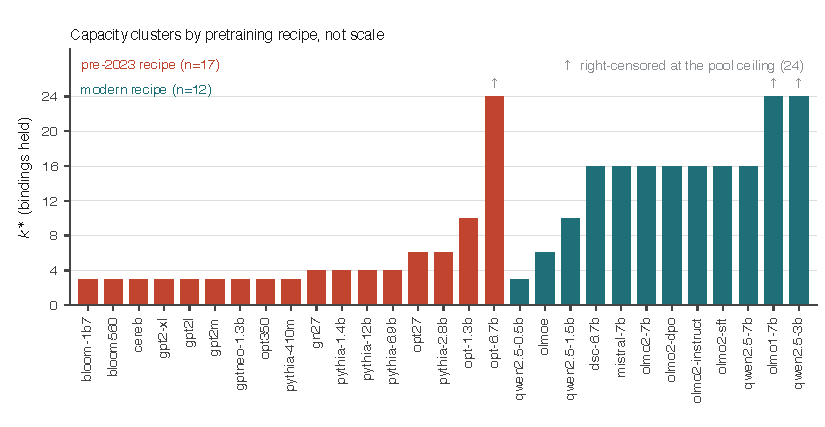
\includegraphics[width=\linewidth]{fig5_capacity.pdf}
  \caption{\textbf{Binding capacity $\kstar$ clusters by pretraining recipe.} Median $\kstar$ is $\KstarOldMed$ for old
  recipes and $\KstarModMed$ for modern ones (family-clustered $95\%$ CI of the difference $\KstarFamCI$; family-level
  $p=\KstarFamP$). The classes \emph{overlap}: OLMoE (modern) sits at $\KstarOlmoE$ and OPT-6.7B (old) reaches the censored
  ceiling. Arrows mark models right-censored at the entity-pool ceiling ($\kstar=\KstarMax$). Pythia-70M is excluded:
  its $K=1$ accuracy is $\PythiaSeventyCeiling$ against a chance of $\Chance$, so its $\kstar$ is not a measurement.
  Regenerated from a committed table (\texttt{results/figdata.json}); statistics by
  \texttt{analysis/capacity\_stats.py}.}
  \label{fig:capacity}
\end{figure}

\section{No geometric predictor survives family clustering}\label{sec:geometry}
Capacity has two geometric correlates at the model level. Across the \NModels{} models, $\kstar$ rises with $\ddecl$
(Pearson $r=\DdeclPearson$, Spearman $\rho=\DdeclSpearman$; partial $\DdeclPartial$ controlling for interference) and falls with
pairwise interference (Pearson $r=\OffdiagPearson$; partial $\OffdiagPartial$). Modern recipes show a higher packing efficiency
$\kstar/\ddecl$ (median $\PackModMed$ vs.\ $\PackOldMed$) at lower interference ($\OffdiagModMed$ vs.\ $\OffdiagOldMed$), and every one of these
comparisons is significant at the model level. These numbers suggest a simple picture: old recipes cram entity codes onto overlapping directions and modern recipes spread them, which would connect binding capacity to
the superposition regime of \citet{superposition2505}, where \emph{loss} scales inversely with model dimension
under strong superposition and the degree of superposition is tunable by weight decay. It would also sit
alongside \citet{largercap2605}, who attribute larger models' advantage to reduced gradient interference
on rare tasks.

\paragraph{Thirty models are not thirty independent samples.} They are \emph{ten families}, and Pythia and
OLMo contribute six apiece. A model-level test treats siblings as independent draws. Under a bootstrap clustered on families, and under a family-level test, the picture does not hold.

\begin{center}
\small
\begin{tabular}{@{}lrrcc@{}}
\toprule
quantity & old med. & modern med. & family-clustered $95\%$ CI & family $p$ \\
\midrule
capacity $\kstar$                   & $\KstarOldMed$  & $\KstarModMed$ & $\KstarFamCI$ & $\mathbf{\KstarFamP}$ \\
packing efficiency $\kstar/\ddecl$  & $\PackOldMed$ & $\PackModMed$ & $\PackFamCI$ & $\mathbf{\PackFamP}$ \\
subspace dimension $\ddecl$         & $\DdimOldMed$ & $\DdimModMed$ & $\DdimFamCI$ & $\DbindFamP$ \\
interference                        & $\OffdiagOldMed$ & $\OffdiagModMed$ & $\OffdiagFamCITab$ & $\OffdiagFamP$ \\
\bottomrule
\end{tabular}
\end{center}

\textbf{Of the two \emph{non-tautological} geometric predictors, neither survives.} The clustered interval for
$\ddecl$ touches zero and its family-level test is not significant; the interval for interference touches zero
as well. The only geometric quantity that survives is packing efficiency, and packing efficiency contains
$\kstar$ in its numerator. It is descriptive by construction and cannot be used to \emph{predict} $\kstar$.

We therefore report the capacity law as the result of this paper and \emph{decline to claim a geometric
mechanism}. The model-level $p$-values are the ones a reader will compute from the released table; we report them alongside the family-clustered results. With ten families (six old, four modern), this is a study with less power than
thirty points suggests; the geometric comparisons do not survive it.

\begin{figure}[t]
  \centering
  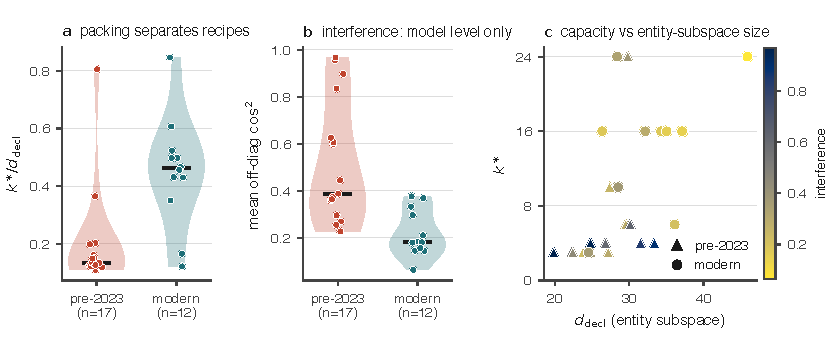
\includegraphics[width=\linewidth]{fig8_recipe.pdf}
  \caption{\textbf{The geometric correlates, at the model level.} \textbf{(a)} Packing efficiency
  $\kstar/\ddecl$ of the declaration-site \emph{entity} subspace and \textbf{(b)} pairwise interference
  separate the recipes at the model level (each point is a model; black dash: median). \textbf{(c)} $\kstar$
  against $\ddecl$ over the \NModels{} measurable models, coloured by interference. Both group comparisons are
  significant at the model level, and \emph{neither non-tautological predictor survives clustering on
  families} (Section~\ref{sec:geometry}); the panels show the model-level pattern in the released table.}
  \label{fig:recipe}
\end{figure}

\section{What this geometry does not explain}\label{sec:notmech}
The packing story could be read as a competitor to the positional-mechanism account of
\citet{mixing2510}, who attribute multi-binding retrieval failure to a positional circuit that grows noisy as
bindings accumulate. We ran the comparison on our own trials, regressing per-trial error on serial position
and on the pairwise overlap of the declaration-site entity vectors. \textbf{The geometry loses.} Once position is controlled,
subspace overlap adds between $\HtHIncLo$ and $\HtHIncHi$ AUROC on all seven models tested; position alone reaches
$\HtHPosAurocLo$--$\HtHPosAurocHi$.

Neither our geometry nor a bare positional pointer predicts \emph{which} distractor is emitted in our
setting: the emitted obligation is the maximum-overlap competitor on $\HtHFoilOvlLo$--$\HtHFoilOvlHi$ of failures against a
$\HtHFoilOvlChance$ chance rate, and a positional neighbour at or below chance. We note that \citet{mixing2510} do predict
the emitted token, with a causal model that combines the positional mechanism with a \emph{lexical} and a
\emph{reflexive} one and reaches $95\%$ agreement with next-token distributions; our head-to-head pits only their positional term against our overlap term, and it is the positional term alone that wins.

So: \emph{across-model} capacity tracks packing efficiency; \emph{within-model, per-trial} error does not. The
cross-model correlation is an observational regularity over \NModels{} models, not a per-trial mechanism.

One caveat on the comparison itself: our error curve is a primacy curve rather than the U-shape of \citet{mixing2510}, because a $\Dblock$-token
distractor block sits between the declarations and the query and destroys recency. The two settings are not
directly comparable.

\section{Capacity is not robustness}\label{sec:robust}
Raw capacity $\kstar$ (how many bindings fit under mild load) and interference-\emph{robustness} (how recall
degrades as the distractor block $D$ grows at fixed $K$) are distinct axes. We sweep $D$ at $K=\RobustK$ for the
eight models with committed curves (Figure~\ref{fig:robust}). Recall at $D=0$ already spans $\RobustDzeroLo$ to
$\RobustDzeroHi$ (median $\RobustDzeroMed$), and the split in \emph{starting level} is exactly the capacity split: the \RobustLowKN{}
models whose $\kstar$ is below $K=\RobustK$ start at $\RobustDzeroLo$--$\RobustLowKDzeroHi$, while the four with
$\kstar\geq16$ start at $\RobustHighKDzeroLo$--$\RobustDzeroHi$ (the 0.5B entry is the Instruct variant of a
base model with $\kstar=3$). By $D=\RobustDmax$ every model sits at $\RobustDendLo$--$\RobustDendHi$ (median
$\RobustDendMed$), and the collapse \emph{rates} do not follow the capacity ranking. A model can therefore
top the capacity ranking yet collapse as fast as the rest once distractors accumulate, or the reverse. This dissociation matters for the interference wall reported by
\citet{pillm2506}, which our $D$-sweep reproduces: robustness is a second property, and it should be measured
separately from capacity.

\begin{figure}[t]
  \centering
  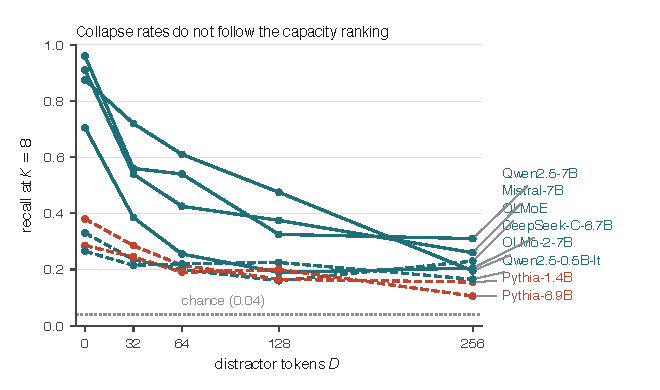
\includegraphics[width=0.8\linewidth]{fig7_robustness.pdf}
  \caption{\textbf{Capacity $\neq$ robustness.} Recall vs.\ interference load $D$ at fixed $K=\RobustK$ for the
  eight models with committed curves (teal: modern recipe; clay: pre-2023). Dashed curves mark the
  \RobustLowKN{} models whose $\kstar$ is below $K=\RobustK$; they start at $\RobustDzeroLo$--$\RobustLowKDzeroHi$
  before any distractor arrives. Collapse rates do not follow the capacity ranking, so robustness is a second
  axis, measured separately.}
  \label{fig:robust}
\end{figure}

\section{Three measurement artifacts, each strong enough to invert the answer}\label{sec:confounds}
Each of these artifacts produces a wrong but plausible-looking number, and each is easy to walk into.

\paragraph{1. Position dominates the raw vectors.} Entity $i$ sits in slot $i$, so declaration-site hidden
states are overwhelmingly positional: the per-slot mean carries $\PosVarLoPct$--$\PosVarHiPct\%$ of their
variance on \GeoNNonOlmo{} of the \GeoNModels{} models with committed geometry; the exception is OLMo-2, at
$\PosVarOlmoPct\%$. A participation ratio taken on the raw vectors reports an effective dimension of at most
$\DrawHi$ and a pairwise squared cosine of $\RawIntLo$--$\RawIntHi$: it is describing \emph{position}.
Estimating the positional component as the per-slot mean across trials and measuring on the residual gives an
interference of $\ResidIntLo$--$\ResidIntHi$ on all \GeoNModels{} models: the entity code is close to
orthogonal to the positional one.

\paragraph{2. Massive activations dominate the covariance.} Once position is removed, a \emph{covariance}
participation ratio is dominated by the residual stream's few massive-activation directions \citep{sink2410}.
It reports an effective dimension of $\DcovQsevenB$ for Qwen2.5-7B, a model that carries $\TopOneQsevenB\%$ of its residual variance
in a single coordinate. Standardizing per coordinate gives $\DdimQsevenB$, and the dimension then scales sensibly with
model size within the family ($\DdimQonefiveB$, $\DdimQsevenB$, $\DdimQfourteenB$ for $1.5$B, $7$B, $14$B).

Both artifacts are \emph{installed by pretraining}. Across Pythia-1.4B checkpoints the positional variance
fraction rises from $\PosVarDevFirst$ to $\PosVarDevLast$ and the top coordinate's share from $\TopOneDevFirst$ to $\TopOneDevLast$, so a measurement
that behaves well on an early checkpoint can invert on a converged one. Under the corrected estimator the
declaration-site subspace does not \emph{compress} over pretraining, as a covariance ratio suggests, but expands
and then plateaus.

\paragraph{3. The site cannot carry a binding.} Most consequential for how the quantity should be read: the
declaration-site vector is taken at the entity token, which causally precedes its obligation. It cannot carry
the binding. The probe numbers in Section~\ref{sec:setup} confirm it: the entity decodes at $1.000$, the obligation at
chance.
$\ddecl$ is therefore the effective dimension of the \emph{entity code}, and the packing-efficiency result is a
statement about how a model spends directions on the entities it must hold apart.

No downstream figure exposes this. The artifact is visible only in the projection of the
declaration-site residuals onto the obligation classes, which gives no separation in any frame, including
a supervised one. A
further provenance caveat: the plotting generator for Figure~\ref{fig:recipe} reads a
committed table, but the \emph{measurement} script that produced the $\ddecl$ values was not preserved, so we
cannot independently verify the token position at which those particular numbers were taken. Re-deriving them at
a position that \emph{can} carry a binding is the correct next measurement: the query site, where the retrieved obligation decodes at $\QueryDecodeLo$--$\QueryDecodeHi$ against a chance of $\Chance$.

\section{Related work}\label{sec:related}
\citet{kim2405} established, on entity tracking with matched base/code-trained pairs, that code pretraining
drives the capability and that alignment tuning adds no consistent benefit; our contribution is the
\emph{quantity}: a named capacity threshold $\kstar$, swept on one instrument across $\NModelsRaw$ models,
with the flat Pythia ladder against an $\KstarRangeFactor\times$ recipe span as the result their
paired-model design could not see. \citet{largercap2605} report per-model entity-capacity breakdowns on two
models; \citet{binding2310} identify the binding-ID mechanism whose fidelity \emph{improves} with scale, an apparent tension with our flat ladder that we leave open: a mechanism's fidelity and a capacity
ceiling can move independently, and a dissociation experiment is the natural next measurement. Two recent
results sharpen the recipe construct. Entity-tracking capacity moves with \emph{architecture} at fixed scale
and data \citep{archentity2606}, so architecture sits inside what we call the recipe; and across a zoo the
same composed-task capability is implemented by different circuits in different models
\citep{mechhet2606}: convergent, from the mechanistic side, with our own finding that no geometric
correlate of $\kstar$ survives family clustering (Section~\ref{sec:geometry}).

\section{Limitations}\label{sec:limits}
\textbf{The law is observational.} The recipe$\to$capacity result is a regularity across \NModelsRaw{} real models, which
differ in data, tokenizer, optimizer, and era simultaneously. The ideal confirmation is a from-scratch causal
ablation: train matched models varying \emph{one} recipe knob and flip $\kstar$. Our attempts were inconclusive
because the from-scratch models were undertrained. We report the observational law; the causal knob remains untested.

\textbf{$\kstar$ is right-censored} at $\KstarMax$ by the entity pool, so the trustworthy signal is the low end.

\textbf{The task is synthetic and single-token}, chosen for control. It is a model of working memory, not a
naturalistic benchmark.

\textbf{The geometry is a correlate, not a mechanism}, and Section~\ref{sec:notmech} reports the head-to-head
it loses. It describes what differs across recipes; it does not predict which trial fails.

\section{Conclusion}
The number of in-context bindings a language model can hold is set by how it was trained, not by how big it
is: a $29\times$ increase in Pythia's parameters moves $\kstar$ from $\PythiaKstarFirst$ to $\PythiaKstarLast$, while the recipe moves the
median from $\KstarOldMed$ to $\KstarModMed$, and that difference survives clustering on families.

The geometry behind the law is not settled by our measurements. Two of its three natural readings are
estimator artifacts (position dominates the raw vectors; massive activations dominate the
covariance), and the third is an artifact of the site: the entity token precedes its obligation, so the
declaration-site vector cannot carry the binding at all. After those corrections, with the ten families clustered, the capacity law survives, the subspace encodes
entities rather than their bindings, and the two geometric correlates have confidence intervals that touch
zero.

\section*{Reproducibility Statement}
Code, data, and the paper source are public at
\url{https://github.com/RavulapalliManas/paper-binding-capacity}: the released capacity table and robustness
curves every figure reads (\texttt{results/figdata.json}), the statistics pipeline
(\texttt{analysis/capacity\_stats.py}), the figure generators (\texttt{figs/gen\_capacity\_figs.py}), and the
macro pipeline that emits every number in this paper's prose from a committed file
(\texttt{analysis/make\_numbers.py} regenerates \texttt{numbers.tex} byte-for-byte). All models are frozen
public checkpoints; the task and the capacity statistic are specified in Section~\ref{sec:setup}. The two open
provenance items are stated where they arise: the full recall-versus-$K$ curves
(Section~\ref{sec:setup}; the re-measurement runner ships in the repository) and the unpreserved $\ddecl$
measurement script (Section~\ref{sec:confounds}).

\bibliographystyle{plainnat}
\begin{thebibliography}{99}

\bibitem[Gu et al.(2025)]{sink2410}
X.~Gu et al. When attention sink emerges in language models: an empirical view. \emph{ICLR}, 2025. arXiv:2410.10781.

\bibitem[Feng and Steinhardt(2024)]{binding2310}
J.~Feng and J.~Steinhardt. How do language models bind entities in context? \emph{ICLR}, 2024. arXiv:2310.17191.

\bibitem[Kim et al.(2024)]{kim2405}
N.~Kim, S.~Schuster, and S.~Toshniwal. Code pretraining improves entity tracking abilities of language
models. 2024. arXiv:2405.21068.

\bibitem[Li and Merrill(2026)]{archentity2606}
Y.~Li and W.~Merrill. Comparing transformers and hybrid models at the token level. 2026. arXiv:2606.20936.

\bibitem[Xu(2026)]{mechhet2606}
Y.~Xu. Pattern selectivity is not task-causal structure: a cross-architecture mechanistic study of
composed-task circuits in 1B-class language models. 2026. arXiv:2606.05378.

\bibitem[Gur-Arieh et al.(2026)]{mixing2510}
Y.~Gur-Arieh, M.~Geva, and A.~Geiger. Mixing mechanisms: how language models retrieve bound entities in-context. \emph{ICLR}, 2026. arXiv:2510.06182.

\bibitem[Huang et al.(2026)]{largercap2605}
J.~Huang, S.~Wurgaft, H.~Bansal, L.~Ruis, N.~Saphra, D.~Alvarez-Melis, A.~Lampinen, C.~Potts, and E.~Lubana. Why larger models learn more: effects of capacity, interference, and rare-task retention. 2026. arXiv:2605.29548.

\bibitem[Liu et al.(2025)]{superposition2505}
Y.~Liu, Z.~Liu, and J.~Gore. Superposition yields robust neural scaling. \emph{NeurIPS}, 2025. arXiv:2505.10465.

\bibitem[Schaeffer et al.(2023)]{mirage2304}
R.~Schaeffer, B.~Miranda, and S.~Koyejo. Are emergent abilities of large language models a mirage? \emph{NeurIPS}, 2023. arXiv:2304.15004.

\bibitem[Wang and Sun(2025)]{pillm2506}
C.~Wang and J.~V.~Sun. Unable to forget: proactive interference reveals working memory limits in LLMs beyond context length. 2025. arXiv:2506.08184.

\end{thebibliography}
\end{document}
